\section{Evaluation}
\label{sec:evaluation}

This section describes the evaluation process and presents the results of the evaluation. In order to run the evaluation we created a small Java project called \verb|evaluator|. It contains the classes to evaluate the performance of the recommender discussed in this report and the Top Popular recommender (see section \ref{sec:baseline}). We use the MovieLens data set as training and test data set. Note that this data set contains preference values.

Evaluation is important because:
\begin{itemize}
  \item It allows us to decide if the quality of the recommender engine archives the desired results. 
  \item We are able to compare the discussed approach to other recommender algorithms. It allows us to compare different recommender techniques.
  \item Evaluation allows us to adjust the parameters in order to get better results.
\end{itemize}

\subsection{How to measure the performance of the \gls{topnt}?}

Most commonly accepted evaluation measure for recommender systems is the Mean Average Error or Root \gls{mae} of the predicted ratings and the actual one \cite{Ricci}\cite{jannach11}.
As decribed in section \ref{sec:problem} the \gls{rec} does not estimate preference values. It produces a \glspl{topn}. Hence we can not use \gls{mae} as a performance metric. 

We can look at the recommender problem as a classification problem. The recommender engine assigns every item into the category of recommendable items or unimported items.
If we look at the recommender problem as a classification problem we can make use of precision and recall to evaluate the performance. Precision and \gls{recall} are two \gls{ir} concepts \cite{Manning}. We provide a brief summary here to each of these measures.

Precision and recall depend on the following measures.
\begin{description}
\item[True positive (TP)] Number of items classified as recommendable or relevant that are truly of interest to the user. 
\item[True negatives (TN)] Number of instances not contained in the recommendation list (classified as irrelevant) and that in fact are not of interest to the user.
\item[False positives (FP)] Number of instances recommended but are not relevant to the user.
\item[False negatives (FN)] Number of instances not shown in the recommendation list but that in fact are relevant to the user.
\end{description}


\begin{figure}
\centering
\begin{tikzpicture}[
box/.style={draw,rectangle,minimum size=3cm,text width=2.5cm,align=left}]
\matrix (conmat) [row sep=.1cm,column sep=.1cm] {
\node (tpos) [box,
    label=left:Relevant items,
    label=above:,
    ] {relevant \\ recommendations \\ (TP)};
&
\node (fneg) [box,
    label=above:,
    label=above right:,
    label=right:] {relevant\\ but not \\recommended\\(FN)};
\\
\node (fpos) [box,
    label=left:irrelevant items,
    label=below left:,
    label=below:Top-N list] {irrelevant \\but\\recommended};
&
\node (tneg) [box,
    label=right:,
    label=below:not in Top-N list] {irrelevant\\and not\\recommended};
\\
};
\node [left=.05cm of conmat,text width=1.5cm,align=right] {\textbf{actual \\ prefences}};
\node [above=.05cm of conmat] {\textbf{recommender classification}};
\end{tikzpicture}
\caption{Confusion matrix for top-N recommendation task}
\label{fig:confusionmatrix}
\end{figure}

Figure \ref{fig:confusionmatrix} visualizes the measures used for precision and recall. This table is called confusion matrix or contingency table \cite{Manning}. 

\subsubsection{Precision and Recall}
\label{sec:precision}

\begin{description}
\item[Precision] Precision is the proportion of items in the top-N list of recommendatoins that are relevant \cite{Manning}.
  \begin{equation}
    \label{eq:precision}
    \text{Precision} = \frac{\text{number relevant items recommended}}{\text{size of the recommendation list}}
  \end{equation}
We can formulate this with the measures from the confusion matrix.
  \begin{equation}
    \label{eq:precisionm}
    \text{Precision} = TP/(TP+FP)
  \end{equation}

 Suppose the recommender create a list of 5 items. If 3 items are relevant recommendations then the precision is $3/5$. 
Precsion only considers the accuracy of the recommendation list and not the comprehensiveness of the result.

\item[Recall] Recall is the proportion of relevant items that appear in the recommendation result. 
  \begin{equation}
    \label{eq:recall}
    \text{Recall} = \frac{\text{number relevant items recommended}}{\text{relevant items}}
  \end{equation}
  \begin{equation}
    \label{eq:recallcm}
    \text{Recall} = TP/(TP+FN)
  \end{equation}
Suppose there are 9 relevant recommendations. If the recommender results contains 3 of these relevant recommendations then the recall is 3/9.

Note that recall should not used without precision. We could build a recommender with perfect recall by recommending all items.
\end{description}

\subsubsection{Implementation}
\label{sec:irimpl}

Listing \ref{lst:irstats} shows the implementation of precision and recall. 
The variable \verb|rec| contains an object of type \verb|Recommender|. \verb|Recommender| provides the method \verb|recommend|. \verb|recommend| takes the ID of the active user and the size $N$ of the top-N list as parameters. The argument \verb|topNsize| corresponds to $TP+FP$. It returns a top-N list for the active user. 

The variable \verb|relevantItemIDs| contains a list with relevant items for the active user.

We count how many items in the top-N list are also in the list \verb|relevantItems| and assign the result in \verb|relevantItemsRetrieved|. \verb|relevantItemsRetrieved| corresponds to the $TP$ value. In order or compute precision or recall we divide \verb|relevantItemsRetrieved| by \verb|topNsize| or the size of the collection\\ \verb|relevantItems|.


\begin{lstlisting}[caption=Implementation of precision and recall,label=lst:irstats]
double precision = 0;
double recall = 0;
int relevantItemsRetrieved = 0;

List<RecommendedItem> recItems = rec.recommend(userID, topNsize);
   for (RecommendedItem recItem : recItems) {
	if (relevantItem.contains(recItem.getItemID())){
			relevantItemsRetrieved++;
	}
   }

// Precision
int numRecommendedItems = reItems.size();
precision = ((double) relevantItemsRetrieved / (double) topNsize);
		      
// Recall
recall =  relevantItemsRetrieved / (double) relevantItems.size());
		      
\end{lstlisting}

\subsection{Testing Methodology}
\label{sec:methodology}
The definitions \ref{eq:precision} and \ref{eq:recall} of precision in recall rely on the number of relevant items.
If we want to evaluate a recommender with \gls{precision} and \gls{recall}, we have to define, what is a relevant item for the active user. 

Relevancy depends on the goal of the recommender. For example, an item is relevant if the user would give it a high rating or if he would purchase the item but he is not aware of it.
Those items are unknown at the time of the recommendation. 

Unfortunatly we do not know if a user likes some new item in the future.
But we can simulate the prefencences of the future by setting aside a small part of the real data set as test data.

In order to separate the test data set from the training data set we get all ratings of user $u$. We sort these rating according the rating value. Then we select the top $N$ items $T$ that are greater then a given threshhold $t$ from the sorted list. Items in $T$ have a high rating and we assume they are relevant to the user $u$. Items in $T$ form the set $TP + FN$ (see figure \ref{fig:confusionmatrix}). 
The threshhold prevents us from adding items with a low rating to $T$. If a user rates three items with the rating 5.0, 1.0 and 1.0 the evaluation algorithm would add the items with the bad rating 1.0 to $T$. Hence the items with bad rating 1.0 lead to lower recall measures. 
If there are no numerical rating values but only Boolean values we have to select $N$ items at random.

All ratings in $T$ are removed from the overall input set. The remaining preferences form the training data set $M$. In order to measure precision and recall we first train the recommender with the data in $M$. For instance, if we evaluate a co-occurence based recommender we compute indicator matrix from section \ref{sec:llr} with this set.

We use the trained recommender to form the \gls{topn} for user $u$. This list corresponds to the set $TP + FP$ in the confusionmatrix.

We check how many items are contained in the top-N list that are in $T$. These items are the set $TP$ (see figure \ref{fig:confusionmatrix}). 

For example, if $N$ is 5 this would mean \gls{precision} and \gls{recall} are evaluated by removing the top 5 preferences for a user and then finding the percentage of those 5 items included in the top-N recommendation list for that user. 

In short the evaluatuation process for a single user $u$ can be devided into several steps:
\begin{enumerate}
\item Retrieve relevant items $T$ for user $u$ ($TP+FN$).
\item Build the training set $M$ by removing the corresponding preferences from input data set.
\item Train the recommender engine with $M$.
\item Form a \gls{topn} for $u$ ($TP+FP$).
\item Count the number of items that appear in the top-N list and in $T$ ($TP$).
\item Compute precision and recall based on $TP$, $FP$ and $FN$.
\end{enumerate}

The evaluation process has the following parameters:
\begin{description}
\item[Size of the result] The length $N$ of recommendations list and number of the relevant items. 
\item[Relevance threshold] Determines if an item is relevant or not.
\end{description}

\subsection{Baseline algorithms}
\label{sec:baseline}

In order to get a feel what values of precision an recall to excpect and to determine the performance of the search engine based, multimodal recommender we compare it with three base line algorithms. 

\begin{description}
\item[Random] The recommender randomly recommends $N$ items to the user. This algorithms serves just as baseline for the more complex algorithms.
\item[Top popular]  It creates a list of items ordered by the numbers of ratings for a specific item. Top Popular is a non-personalized recommender because it presents the same list of items to any user \cite{Cremonesi}. Listing \ref{lst:toppop} shows the implementation of the the Top Popular algorithm. 

\begin{lstlisting}[label=lst:toppop, caption={Implementation of top popular recommender}]
Map<Long, Integer> item2pop = new HashMap<Long, Integer>();
LongPrimitiveIterator iter = dataModel.getUserIDs();
while (iter.hasNext()) {
PreferenceArray prefs = dataModel.getPreferencesFromUser(iter
	.nextLong());
for (int i = 0; i < prefs.length(); i++) {
	Integer counter = item2pop.get(prefs.getItemID(i));
	if (counter == null) {
		item2pop.put(prefs.getItemID(i), 1);
	} else {
		item2pop.put(prefs.getItemID(i), counter + 1);
	}
      }
}
List<RecommendedItem> popitems = transfom2list(item2pop);
Collections.sort(itemidcounter, new RecommenderItemComparator()); 
return popitems
\end{lstlisting}

\item[Item-based with cosine similarity]  \Gls{itembased} collaborativ filtering is a model-based, collaborative filtering algorithm. It computes the simililarities between all items and predicts user prefences by based one existing ratings. We use the cosine similarity \cite{ekstrand11} to measure the similarity between two items. The \gls{itembased} algorithm selects $k$ neirest neighbors $N$ of $i$. It then weights the ratings of the active user $u$ for each item $i'$ in $N$ with the similarity $sim(i,i')$ and compute the sum of that. The predicted rating $r_{u,i}$ for user $u$ and item $i$ is the normalized value of the sum \cite{jannach11}:

\end{description}
\begin{equation}
  \label{eq:computeprediction}
  r_{u,i} = \frac{\sum_{i' \in N}{sim(i,i') r_{u,i}}}{\sum_{i' \in N}{|s(i,i')|}}
\end{equation}

We use Mahouts implementation of an \gls{itembased} recommender. Mahout provides the \verb|GenericItemBasedRecommender| class with an implementation of an \gls{itembased} recommender. To compute the similiarty we use \verb|UncenteredCosineSimilarity|.

\subsection{Dataset}
\label{sec:dataset}

The testing methodology of section \ref{sec:methodology} requires an existing data set. We used ratings and tagging activity from MovieLens, a movie recommendation service \cite{movielensdata}.
MovieLens data sets were collected by the GroupLens Research Project at the University of Minnesota. The data was collected through the MovieLens web site (movielens.umn.edu) during the seven-month period from September 19th, 1997 through April 22nd, 1998 \cite{movielensdata}.

This data set consists of:
\begin{itemize}
\item 100,000 ratings. The ratings are scores from 1 to 5. A rating is made by one user to one movie at a specific time. 

\item 943 users. Each user has rated at least 20 movies
\item 1682 movies. Movies are categorized in genres. A movie has an ID, a title, and a list of associated genres. 
\item 2488 \gls{tag} appliciations. A \gls{tag} is applied by one user to one movie at a specific time. Tags are user-generated metadata about movies. Each tag is typically a single word or short phrase. The meaning, value, and purpose of a particular tag is determined by each user.
\end{itemize}
 
We choose this dataset due to several reasons:
\begin{itemize}
\item It contains ratings and tagging activity. Hence we can use two indicators for the multimodal co-occurence based recommender.
\item As described in section \ref{sec:methodology} we need numerical rating scores to select the top $N$ ratings of a user in order to form a test set. 
\item  It is common to evaluate a recommender engine with it. Hence it is easier to compare the results with other recommender engines. 
\end{itemize}

The co-occurence based recommender takes user actions as Boolean values as an input. The MovieLens data set contains preferences with a numerical rating score. 
In order to simulate the user action ``like'' as described in section \ref{sec:inputdata} we generate a new data set based on the MovieLens data set. We select all preferences with a score equal or above 4.0. These \glspl{preference} indicate that the user likes the item hence we consider them as likes.

\subsection{Evaluationresults}
\label{sec:results}
To compare the \gls{rec} with the baseline algorithms (described in section \ref{sec:baseline}) we use three \glspl{indicator}.

\begin{description}
\item[Co-occurence user likes] As described in section \ref{sec:dataset} we generate a user action history with ``like'' actions. We calculate the \gls{llr} strengths between all items and use the rrecent likes in the user's history as query.
\item[User ratings] We use the \gls{coocc} based similiarity metric descibed in section \ref{sec:}the preference values to calculate the  similarity between all items.
\item[Tags] We use the tags associated with an item to compute a tag \gls{indicator} matrix. We use the tags associated with the user to create a query.
\end{description}

We created three recommenders. We measure precision and recall first with the recommender ``1.indicator'' that only considers co-occurence of user likes. Then we add the indicator ``user ratings'' to the multimodal recommender ``2 indicators'' and then we use all 3 indicators to retieve a \gls{topn} (``3. indicators''). 

We measure precision and recall at $N=10$. Hence we retrieve a list of 10 items. Relevant items are the 5 best rated items above a threshold of $\mu + \sigma$ all user ratings.

\pgfplotsset{width=7cm}
\begin{figure}
  \centering
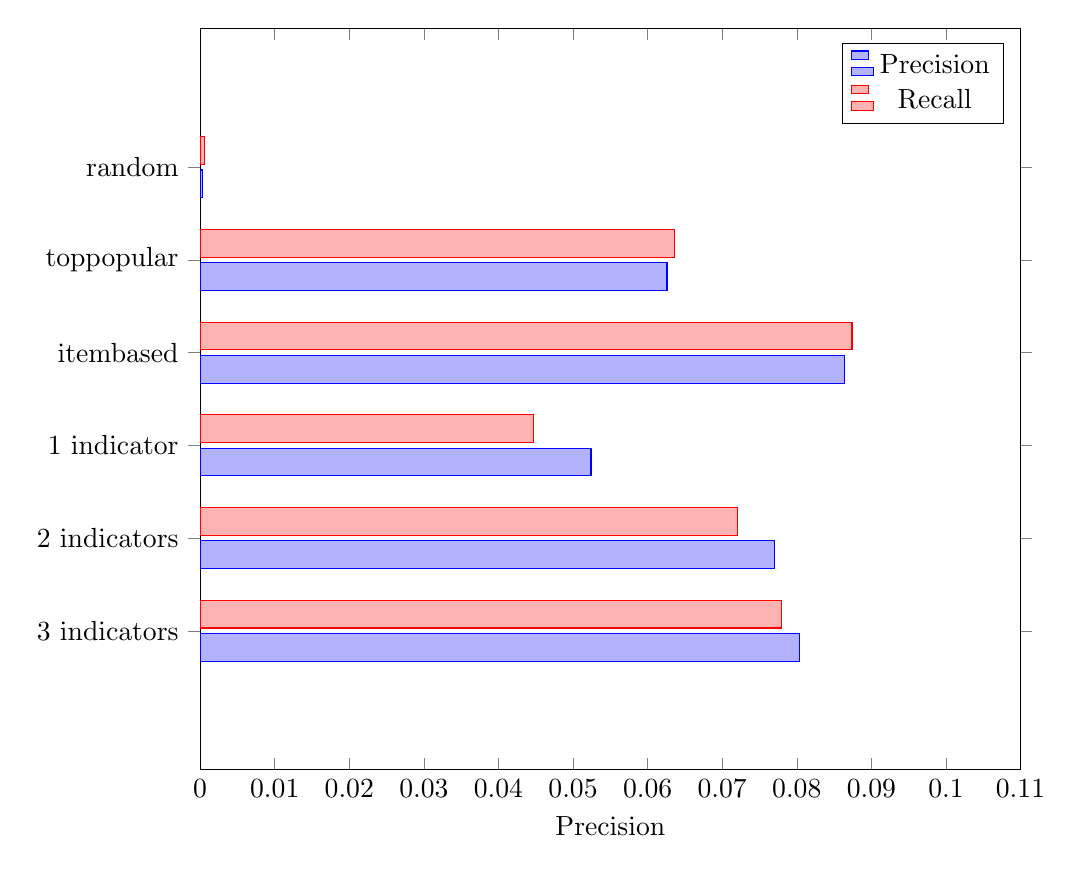
\begin{tikzpicture}
\begin{axis}[
xbar,
xmin=0,
xmax=0.11,
width=12cm,
height=11cm,
enlarge y limits=0.3,
xlabel={Precision},
symbolic y coords={3 indicators,2 indicators,1 indicator,itembased,toppopular,random},
ytick=data,
x tick label style={/pgf/number format/fixed}
]

\addplot coordinates {(0.00035,random) (0.0626,toppopular) (0.0864,itembased) (0.0524,1 indicator) (0.077,2 indicators) (0.0804,3 indicators)};
\addplot coordinates {(0.00054,random) (0.0636,toppopular) (0.0874,itembased) (0.0447,1 indicator) (0.072,2 indicators) (0.078,3 indicators)};
\legend{Precision, Recall};
\end{axis}
\end{tikzpicture} 
\caption{Precision comparison of recommender algorithsm, random generated recommendations, Top Popular and itembased with precision at 10 and $N$ = 10 (number of recommended items)}
  \label{fig:precisionrecallvalues}
\end{figure}

Figure \ref{fig:precisionrecallvalues} shows the comparison of \gls{coocc} based recommender with one, two and three indicators with the baseline algorithms from section \ref{sec:baseline}.
The multimodal co-coccurence  achieves an average precision and recall of 8 and 7.8 percent. This seems low. The recommender rarely recommends an item that the user liked explicitly. On the other hand we do not know if the recommended items are appealing to the user if he never rated them.

The evaluation shows that the quality of the recommender increases when we take more indicators into account. If we use just the user action ``like'' precision and recall are 5.2 and 4.5 percent. If we use user ratings and tags as indicator precision and recall are  8 and 7.8 percent. That an increase of 53 and 73 percent.

Compared to the baseline algorithms the \gls{coocc} based recommender achieves the second best results. It performs better than the non-personalized TopPopular algorithm and slightly worse than the itembased algorithm. The reason for this is the lack of a relevancy score for the similarities. The itembased algorithms considers the similirity value. The search engine does not have this information. Either a item id is part of a indicator field or not. This circumstance could be improved by using payloads in Solr. Another interesting fact is that the non-personalized algorithm almost match the quality of the more sophisticated approaches. Compared to randomly generated recommendations the \gls{coocc} improves the quality with a factor of about 250.
